% LyX 2.0.5.1 created this file.  For more info, see http://www.lyx.org/.
% Do not edit unless you really know what you are doing.
\documentclass[12pt,english]{report}
\usepackage{mathptmx}
\renewcommand{\familydefault}{\rmdefault}
\usepackage[T1]{fontenc}
\usepackage[latin9]{inputenc}
\usepackage[a4paper]{geometry}
\setcounter{secnumdepth}{2} % Changed from 3 to 2. 0-chapter 1-section 2-subsection 
\setcounter{tocdepth}{2} % Changed from 3 to 2. 0-chapter 1-section 2-subsection 
\setlength{\parskip}{\medskipamount}
\setlength{\parindent}{0pt}
\usepackage{verbatim}
\usepackage{pdfpages}
\usepackage{graphicx}
\usepackage{subfig} %% This package has to be here
\usepackage{setspace}
\usepackage{arabtex}
\usepackage[numbers]{natbib}
\usepackage{nomencl}
\usepackage{amsthm}
\usepackage{amsmath}
\usepackage{amsfonts}
\usepackage{etoolbox}
\newtoggle{edit-mode}
\toggletrue{edit-mode}  
%\toggletrue{edit-mode}
\iftoggle{edit-mode}{
\geometry{verbose,tmargin=2cm,bmargin=2cm,lmargin=2cm,rmargin=6cm,headheight=1cm,headsep=1cm,footskip=1cm, marginparwidth=5cm}
}{
\geometry{verbose,tmargin=2cm,bmargin=2cm,lmargin=2cm,rmargin=2cm,headheight=1cm,headsep=1cm,footskip=1cm}
}

\makenomenclature

% Theorem Styles
\newtheorem{theorem}{Theorem}[section]
% Definition Styles
\theoremstyle{definition}
\newtheorem{definition}{Definition}[section]
\newtheorem{example}{Example}[section]
\theoremstyle{remark}
\newtheorem{remark}{Remark}

\usepackage[linesnumbered]{algorithm2e}

\begin{document}
\printnomenclature{}

\tableofcontents{}

%Instructions - How to write a background:
%-------------------------------------------------
%Incorporating background information into the Introduction is intended to provide the reader with critical information about the topic being studied, such as highlighting and expanding upon foundational studies conducted in the past, important historical events that inform why and in what ways the research problem exists, or defining key components of your study [concepts, people, places, things]. Although in  social sciences research introductory background information can often blend into the literature review portion of the paper, basic background information should not be considered a substitute for a comprehensive review and synthesis of relevant research literature.
%Providing background information in the Introduction of a research paper serves as a bridge that links the reader to the topic of your study. But precisely how long and in-depth this bridge should be is largely dependent upon how much information you think the reader will need in order to understand the research problem being discussed and to appreciate why the issues you are investigating are important.
%From another perspective, the length and detail of background information also depends on the degree to which you need to demonstrate to your professor how much you understand the topic. Keep this in mind because providing succinct background information can be an effective way to show that you have a clear grasp of key issues and concepts underpinning your overall study. Don't try to show off, though!
%Given that the structure and writing style of your background information can vary depending upon the complexity of your research and/or the nature of the assignment, here are some questions to consider while writing:
%1. Are there concepts, terms, theories, or ideas that may be unfamiliar to the reader and, thus, require additional explanation?
%2. Are there historical elements that need to be explored in order to add needed context, to highlight specific people, issues, or events, or to lay a foundation for understanding the emergence of a current issue or event?
%3. Is the research study unusual in some way that requres additional explanation, such as, 1) your study uses a method never applied before to the research problem you are investigating; 2) your study investigates a very esoteric or complex research problem; or, 3) your study relies upon analyzing unique texts or documents, such as archival materials or primary documents like diaries or personal letters, that do not represent the established body of source literature on the topic.



\chapter{Background}

\section{Handwriting Recognition}

\textbf{MindMap}
\begin{itemize}
\item Talk about OCR in general, and make the distinctions between the following: Handwriting vs. printed, the different types of writing, Open vs. Close dictionary, etc.
\item what is the current status of knowledge about handwriting recognition - general literature review.
\item mention Latin and Chinese in the background.
\end{itemize}


\iftoggle{edit-mode}{\hspace{0pt}\marginpar{Definition and history of OCR}}{}
\emph{Optical character recognition} (OCR) is an electronically converting a scanned, photoed or sensed images of typewritten or printed text into machine-encoded text.
It has been an actively researched since the early days of computers; a 1972 survey cites nearly 130 works on the subject. 
{\color{blue} Historically, optical character recognition was considered a technique for solving a particular kind of pattern recognition problems. Indeed, to recognize a character from a given image, one would match (via some known metric) this character's feature pattern against some very limited reference set of known feature patterns in the given alphabet. This clearly is a classical case of a pattern recognition problem. Character classification has always been a favorite testing ground for new ideas in pattern recognition, but since many such experiments are conducted on isolated characters, the results are not always immediately reflected in OCR applications. Optical character recognition has been steadily evolving during its history, giving rise to an exciting set of research topics and producing many powerful practical applications. Now it is considered one of the best applications of machine vision and one of the most successful research branches in pattern recognition theory. Being a well developed technological field, optical character recognition is widely used today for projects of various scales, from occasional document scanning to creation of massive digital document archives. Yet it remains an area of active scientific research and creative engineering.}

\iftoggle{edit-mode}{\hspace{0pt}\marginpar{Motivation for HWR}}{}
Handwriting recognition (HWR) can be defined as the task of transforming text represented in the spatial form of graphical marks into its symbolic representation. 
Despite long standing predictions that handwriting, and even paper itself, would become obsolete in the age of the digital computer, both persist. 
While much of the today's data is directly entered into computers using the keyboard, many tasks still exist in which people tend to prefer handwriting over keyboard entry.
Whilst the computer has hugely simplified the process of producing printed documents, the convenience of a pen and paper still makes it the natural medium for many important tasks.  
Note taking (e.g. in classrooms) is a task that can still be done more efficiently by hand for most users. 
However, the ease and convenience of having information in digital form provides a powerful incentive to find a way of quickly converting handwritten text into its digital equivalent
Not only is this useful for making digital copies of handwritten documents, but also in many automated processing tasks, such as searching, indexing, automatic mail sorting, cheque processing. 
Smart-phones and tablets devices are too small to have full sized keyboards, or sometimes may be too small for any keyboard at all, requiring pen, hand gestures, figure gestures or voice interface to enter data. 
The problem of handwriting recognition has now been a topic of research for over four decades. 
There are many types of problems (with varying complexity) within handwriting recognition, based on how the data is presented to the recognition system, at what level the data can be unambiguously broke into pieces (e.g. individual characters or words), and the transcription complexity of the language used \cite{burrow2004arabic, connell2000online}. 

\subsection{Types of handwriting input:off-line versus on-line}
Handwriting data is converted to digital form either by scanning the writing on paper or by writing with a special pen on an electronic surface such as a digitizer combined
with a liquid crystal display. The two approaches are distinguished as off-line and on-line handwriting, respectively.
Off-line HWR focuses on documents that have been written on paper at some previous point of time. 
Information is presented to the system in the form of scanned image of the paper document. 
In contrast, on-line HWR, the two-dimensional coordinates of successive points of the writing as a function of time are stored in order, i.e., the order of strokes made by the writer is readily available. 
This requires the use of special equipment, such touch screen or digitizing tablet, to capture the strokes of the pen as that are being written. 
While this sequence can be used to construct a static image of the writing, thus allowing off-line character recognition techniques to be applied, it has been shown that the information about the pen dynamics can be used to obtain a better recognition accuracies than the static data alone. Figure \ref{fig:offlibe_vs_online} shows typical input signals that can be analyzed in both cases.

An advantage of on-line handwritten data over off-line data is the availability of the stroke segmentation and the order of writing. 
Ink in static images must first be separated from the image background, creating a potential source of error. 
The ability to detect the states of "pen-down" (when the pen touches the tablet or the finger touches the touch screen) and "pen-up" can also be used. 
A single stroke is defined as the sequence of sample points occurring between consecutive pen-down and pen-up transitions. 
However, a complication occurs when a stroke is added to a character in a word after the rest of the word has already been written, such as the cross of a 't' or an 'x', or the dot of an 'i' or a 'j' These types are called delayed strokes \cite{connell2000online}. 

%On-line Hand Writing Recognition refers to the situation where the recognition is performed concurrently to the writing process. 

\begin{figure}
	\centering
        \subfloat[]{
            \label{fig:offline}
            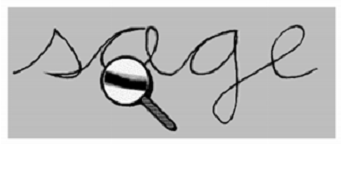
\includegraphics[width=0.5\textwidth]{./figures/offline}
        }
        \subfloat[]{
           \label{fig:online}
           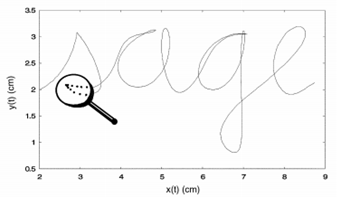
\includegraphics[width=0.5\textwidth]{./figures/online}
        }        
    \caption{(a) Off-line word. The image of the word is converted into gray-level pixels using a scanner. (b) On-line word. The x; y coordinates of the pen-tip are recorded as a function of time with a digitizer}
   \label{fig:offlibe_vs_online}
\end{figure}

\iftoggle{edit-mode}{\hspace{0pt}\marginpar{Types of English texts forms}}{}
Latin handwriting can appear in several forms which impose a different recognition difficulties. The \textbf{cursive script} form, which is the most common type of day-to-day script, is the text in which words, or portion of a word, is written with a single stroke, i.e, ligatures connect adjacent letters. 
The \textbf{hand-printed script} is the case where the writing still represents an entire word sequence, but succeeding characters are explicitly segmented by a pen lift; though, the character segmentation problem is still not solved as pen lifts can also occur within a character. 
Another form is the \textbf{isolated characters} form, in which the segmentation problem is already solved, for instance by the acquisition interface and the cooperation of the writer. 
Graphical boxes or timeouts are common interface techniques for this purpose.
However, in the Arabic language, the only case is the cursive, in both handwritten and printed text.
One problem in unconstrained HWR is the huge variety in the writing of different people. Another extreme difficulty is the so-called segmentation, that is, the process of dividing an entire writing into sub-units (typically characters).
The recognition difficulty decreases from the first listed type to the last. Indeed, HWR systems have a strong history in making use of this graduation in difficulty. They have aimed (and still aim) at a reasonable user satisfaction by restricting the text input to a simpler handwriting type, while simultaneously rewarding the user with recognition accuracy \cite{bahlmann2005advanced}.
After a long period of focus on western and East Asian scripts there is now a general trend to explore other scripts such as Arabic and various Indic scripts. 


\iftoggle{edit-mode}{\hspace{0pt}\marginpar{Closed Vocabulary vs. Open Vocabulary}}{}
{\color{blue}
Vocabulary is also a major factor in determining how difficult a handwriting
recognition task is. Closed-vocabulary tasks refer to recognition of words from a
predetermined dictionary. The dictionary size is arbitrary. Open-vocabulary tasks refer to
recognition of any words without the constraint of being in a dictionary.
Closed-vocabulary tasks are easier than open-vocabulary ones because only certain
subsequences of letters are possible when limited by a dictionary.
Closed-vocabulary tasks using a small dictionary are especially easy because: 1) a -
small vocabulary size can mean a smaller number of configurable word pairs; 2) a small
vocabulary size enables the direct modeling of individual words, whereas a large
vocabulary size necessitates the modeling of letters, which is due to the computational
complexity of modeling words directly, 3) with the usage of letters for large vocabulary
tasks, the search space of all possible sentences i usually much larger due to an increase in
the number of nodes in the search graph. When letters are used for modeling instead of
words, the number of nodes is $mxn$ instead of n where as the number of words, and m
is the average number of letters per word (generally between three and ten).
As the vocabulary size increases, the occurrence of out-of-vocabulary words is
less frequent. Thus, the performance of the large vocabulary tasks is approximately the
same as of the performance of the open-vocabulary tasks.\cite{shu1996line}}


\iftoggle{edit-mode}{\hspace{0pt}\marginpar{Approaches of OCR}}{}


{\color{blue}
%There exist a wide variety of approaches to optical character recognition. Some of them require pre-segmentation into recognition items, and some of them do not, but we can safely expect that any OCR algorithm would posses these two essential components:
%\begin{itemize}
%\item a feature extractor, and
%\item a classifier
%\end{itemize}
%Given an item image, the feature extractor derives the features (descriptors) that the item possesses. The derived features are then used as input to the classifier that determines the (most likely) known item corre sponding to the observed features. The classifier is also expected to give a confidence level number that tells how certain the classifier is about the recognized item. }
%
%


\emph{see: \cite{al2010development} section "types of handwriting input - on-line and off-line"}

\emph{TODO: for online handwriting recognition see for all these sections see H. Shu, "On-line handwriting recognition using hidden Markov models," 1996.}


\subsection{Handwriting Segmentation}
{An integralpartofthehandwritingrecognitionprocessis
segmentation. Thetechniquerequiresanover-segmentationstage
which partitionhandwrittenwordsintoprimitivesthatmaythen
be processedfurthertoprovidethebestsegmentation.}


%%%%%%%%%%%%%%%%%%%%%%%%%%%%%%%%%%%%%%%%%%%%%%%%%%%%%%%
\newpage{}
%%%%%%%%%%%%%%%%%%%%%%%%%%%%%%%%%%%%%%%%%%%%%%%%%%%%%%%

\section{Arabic Handwriting Recognition}

\begin{itemize}
\item The Arabic language - Importance and history.
\item Arabic handwriting recognition - Talk about the characteristics of the Arabic script. maybe a little bit of history.
\item Where is does the current knowledge on Arabic handwriting recognition stands - general literature review.
\item Arabic segmentation
\end{itemize}


\emph{TODO:see the in introduction of \cite{abandah2009analysis}}

\subsection{Characteristic of the Arabic writing system}
\emph{[See Online handwriting recognition for the Arabic Letter Set]}
\emph{[See [1]	G. a. Abandah and M. Z. Khedher, "Analysis of Handwritten Arabic Letters Using Selected Feature Extraction Techniques,"International Journal of Computer Processing of Languages, vol. 22, no. 01, pp. 49-73, Mar. 2009.]}




One difficulty with the Arabic script is the number and position of diacritic marks associated to Arabic characters.

{\color{blue}The Arabic language is one of the most structured and served languages. It comes as the fifth of the most used languages (as a first language) after Chinese, Hindi, Spanish and English. It is spoken as a first language by nearly 350 million people around the globe, mainly in the Arab countries, which is about 5.5\% of the world population (the world population is estimated at 6.44 billion in July 2005) (CIA, 2005). However, almost all Muslims (close to $1/4$ of the world population) can read Arabic script as it is the language of the Holy Qur'an. The Arabic script evolved from a type of Aramaic, with the earliest known document dating from 512 AD. The Aramaic language has fewer consonants than Arabic (Burrow, 2004). The old Arabic was written without dots or diacritics. The dots were first introduced by Yahya bin Ya'mur (died around 746 AD) and Nasr bin Asim (died around 707 AD), students of Abu Al-Aswad Al-Du'ali (died around 688 AD) who introduced the diacritics to prevent the Qur'an from being misread by Muslims (Al-Fakhri, 1997). Figure 1 shows a sample of an old manuscript of a sentence written without dots or diacritics. Due to the Islamic conquests, the use of Arabic language extended in the 7th and 8th centuries from India to the Atlantic Ocean (Al- Fakhri, 1997). Consequently, many other languages adopted the Arabic alphabet with some changes. Among those languages are Jawi, Urdu, Persian, Ottoman, Kashmiri, Punjabi, Dari, Pashto, Adighe, Baluchi, Ingush, Kazakh, Uzbek, Kyrgyz, Uygur, Sindhi, Lahnda, Hausa, Berber, Comorian, Mandinka, Wolof, Dargwa, and few others. Figure 2 shows samples of some of the above mentioned languages. However, it must be mentioned that some of those languages are currently using Latin characters, but in general, people can still read the Arabic script. It is also worth mentioning that the United Nation adopted Arabic in 1974 as its sixth official language (Strange, 1993). Despite the fact that Arabic alphabets are used in many languages, Arabic Character Recognition (ACR) has not received enough interests from researchers. Little research progress has been achieved as compared to the one done on Latin or Chinese. It has almost only started in 1975 by Nazif (1975), while the earlier research efforts in Latin may be traced back to the middle of the 1940s. However, due to a lack of computing power, no significant work was performed until the 1980s. Recent years have shown a considerable increase in the number of research papers related to ACR. (Segmentation of Arabic Characters: A Comprehensive Survey)}\\

The Arabic Aleph bet is widely used for more than twenty different languages such as Farsi, Urdu, Malay, Housa and Ottoman Turkish. Arabic is used in over 20 different countries, written by more than 100 million people and spoken by 234 million people. Although the spoken Arabic is slightly different from country to country, the written Arabic is standard system used all over the Arab world \cite{saabni2009efficient} \cite{jannoud2007automatic}.
Arabic Scripts consists of 28 basic letters, 12 additional special letters, and 8 diacritics. Arabic script is written from right to left in a semi-cursive manner in both printed and handwritten. Most letters are written in four different letter shapes depending on their position in a word, e.g., the letter \RL{`}  (Ain) appears as \RL{`} (isolated), \RL{`-}(initial),\RL{-`-} (medial) and \RL{-`} (final). Among the basic letters, six are Disconnective - \RL{A} (Alef), \RL{d} (Dal), \RL{_d} (Thal), \RL{r} (Reh), \RL{z} (Zain) and \RL{w} (Waw). Disconnective letters do not connect to the following letter and have only two shapes each. The presence of this letters interrupts the continuity of the graphic form of a word. We denote connected letters in a word, as word-part. If the word-part is composed of only one letter, this letter will be in its isolated shape \cite{biadsy2011segmentation}. 
Certain characteristics relating to the obligatory dots and strokes of the Arabic script distinguish it from Roman script, making the recognition of words in Arabic more difficult than in Roman script. First, Most Arabic letters contain dots in addition to the letter body, such as \RL{s} (Sheen) which consists of \RL{s} (Seen) body and three dots above it. In addition to dots, there are stroke that can attach to a letter body creating new letter such as \RL{k}, \RL{.t} and \RL{lA}. These dots and strokes are called delayed strokes since they are usually drawn last in the in handwritten word-part/word. Second, eliminating, adding or moving a dot or stroke could produce a completely different letter and, as a result, produce a word other than the one that was intended (see Table 1). Third, the number of possible variations of delayed strokes is greater than those in Roman scripts, as shown in Figure 2. There are only three such strokes used for English: the cross in the letter t, the slash in x, and the dots in i and j. 

{\color{blue}The Arabic language has some diacritics that are used in the holy book Qur'an and sometimes in teaching material and poetry. These diacritics are small markings used above or below the letters of a word to specify the exact pronunciation of the word. They are not commonly used in the daily, scientific, and business uses, and are not discussed further in this work.(Abandah \& Khedher, 2009)}

{\color{blue}Arabic is written by more than 100 million people, in over 20 different countries.
The Arabic script evolved from a type of Aramaic, with the earliest known document
dating from 512 AD. The Aramaic language has fewer consonants than
Arabic, so new letters were created around the 7th century by adding dots to
existing letters. There are therefore several letters differing only by a single dot.
Other small marks (diacritics) are used to indicate short vowels, but are often
not used. \cite{burrow2004arabic}}


Finally, in Arabic script a top-down writing style called vertical ligatures is very common - letters in a word may be written above their consequent letters. In this style, the position of letters cannot be predefined relative to the baseline of the word \cite{biadsy2011segmentation}.    
Saabni and El-sana have explored a large collection of Arabic texts and extracted 300,000 different word combinations of 82,000 different word-parts. Ignoring the additional strokes reduced the number of different word-parts to 40,000 \cite{saabni2009efficient}. 

\emph{TODO: see the section "Overview of Arabic Letters" in \cite{abandah2009analysis}. It talks about letters frequencies and special letters}

\emph{TODO: talk about the WP and give statistics of WP length as described in {abandah2009analysis}}

\subsection{Issues with Arabic Handwriting Recognition}
{RecognitionandsegmentationofArabichandwrittenscriptisadifficulttaskbecausetheArabic
handwrittencharactersarenaturallybothcursiveandunconstrained.TheanalysisofArabicscriptis
more complicatedincomparisonwithEnglishscript. Itisbelieved,goodsegmentationisonereasonfor
high accuracycharacterrecognition.\cite{al2010development}}

\section{On-line handwriting as temporal information}
\iftoggle{edit-mode}{\hspace{0pt}\marginpar{Online HW representation}}{}

\iftoggle{edit-mode}{\hspace{0pt}\marginpar{Online HW space definition}}{}
The stroke trajectory space definition.

\iftoggle{edit-mode}{\hspace{0pt}\marginpar{Online HW as time series}}{}
However in this work we do not use the temporal information of the written stroke trajectory, however we view it as an ordered set of points. 


\iftoggle{edit-mode}{\hspace{0pt}\marginpar{techniques that were adopted from temporal data classification}}{}


\bibliographystyle{plainnat}
\bibliography{references}
\end{document}
